% Data Flow Diagrams for Multi-Agent JSSP Frameworks
% Generated for research paper

\documentclass{article}
\usepackage{tikz}
\usepackage{pgfplots}
\usetikzlibrary{shapes,arrows,positioning,fit,backgrounds}
\usepackage{geometry}
\geometry{a4paper, margin=1in}

\begin{document}

% MAPLE Data Flow
\begin{figure}[h!]
\centering
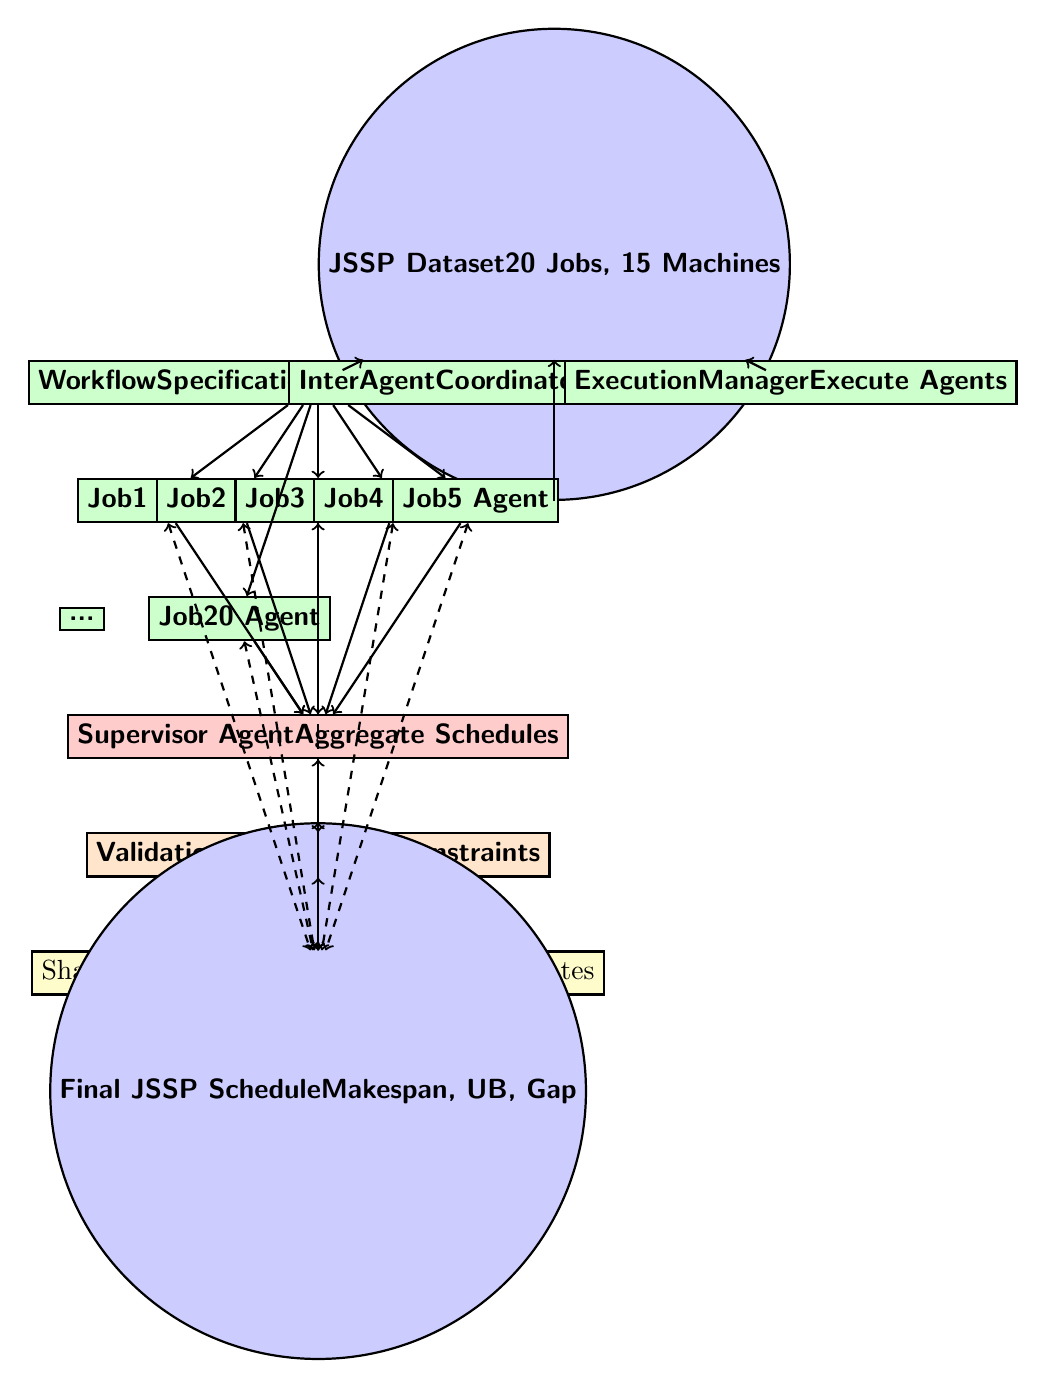
\begin{tikzpicture}[
    node distance=1.5cm,
    auto,
    thick,
    main node/.style={circle,fill=blue!20,draw,font=\sffamily\bfseries},
    agent node/.style={rectangle,fill=green!20,draw,font=\sffamily\bfseries},
    supervisor node/.style={rectangle,fill=red!20,draw,font=\sffamily\bfseries},
    validation node/.style={rectangle,fill=orange!20,draw,font=\sffamily\bfseries}
]

% Input
\node[main node] (input) {JSSP Dataset\\20 Jobs, 15 Machines};

% Layer 1: Specification Construction
\node[agent node, below of=input, xshift=-3cm] (spec) {WorkflowSpecification\\Build Workflow Graph};
\node[agent node, below of=input, xshift=0cm] (coord) {InterAgentCoordinator\\Set Dependencies};
\node[agent node, below of=input, xshift=3cm] (exec) {ExecutionManager\\Execute Agents};

% Job Agents (20 agents)
\node[agent node, below of=spec, xshift=-2cm] (job1) {Job1 Agent};
\node[agent node, below of=spec, xshift=-1cm] (job2) {Job2 Agent};
\node[agent node, below of=spec, xshift=0cm] (job3) {Job3 Agent};
\node[agent node, below of=spec, xshift=1cm] (job4) {Job4 Agent};
\node[agent node, below of=spec, xshift=2cm] (job5) {Job5 Agent};
\node[agent node, below of=job1, xshift=-1cm] (jobdots) {...};
\node[agent node, below of=job2, xshift=0cm] (job20) {Job20 Agent};

% Supervisor Agent
\node[supervisor node, below of=job20, xshift=1cm] (supervisor) {Supervisor Agent\\Aggregate Schedules};

% Validation Agent
\node[validation node, below of=supervisor, xshift=0cm] (validation) {Validation Agent\\Check Constraints};

% Context sharing
\node[draw,rectangle,fill=yellow!20,below of=validation, xshift=0cm, minimum width=4cm] (context) {Shared Context Dictionary\\Real-time Updates};

% Output
\node[main node, below of=context] (output) {Final JSSP Schedule\\Makespan, UB, Gap};

% Arrows
\draw[->] (input) -- (spec);
\draw[->] (input) -- (coord);
\draw[->] (input) -- (exec);

\draw[->] (spec) -- (job1);
\draw[->] (spec) -- (job2);
\draw[->] (spec) -- (job3);
\draw[->] (spec) -- (job4);
\draw[->] (spec) -- (job5);
\draw[->] (spec) -- (job20);

\draw[->] (job1) -- (supervisor);
\draw[->] (job2) -- (supervisor);
\draw[->] (job3) -- (supervisor);
\draw[->] (job4) -- (supervisor);
\draw[->] (job5) -- (supervisor);
\draw[->] (job20) -- (supervisor);

\draw[->] (supervisor) -- (validation);
\draw[->] (validation) -- (context);
\draw[->] (context) -- (output);

% Context sharing arrows
\draw[<->,dashed] (job1) -- (context);
\draw[<->,dashed] (job2) -- (context);
\draw[<->,dashed] (job3) -- (context);
\draw[<->,dashed] (job4) -- (context);
\draw[<->,dashed] (job5) -- (context);
\draw[<->,dashed] (job20) -- (context);
\draw[<->,dashed] (supervisor) -- (context);
\draw[<->,dashed] (validation) -- (context);

\end{tikzpicture}
\caption{MAPLE Data Flow: 3-Layer Architecture with 22 Agents (20 Job + 1 Supervisor + 1 Validation)}
\label{fig:maple_dataflow}
\end{figure}

% CrewAI Data Flow
\begin{figure}[h!]
\centering
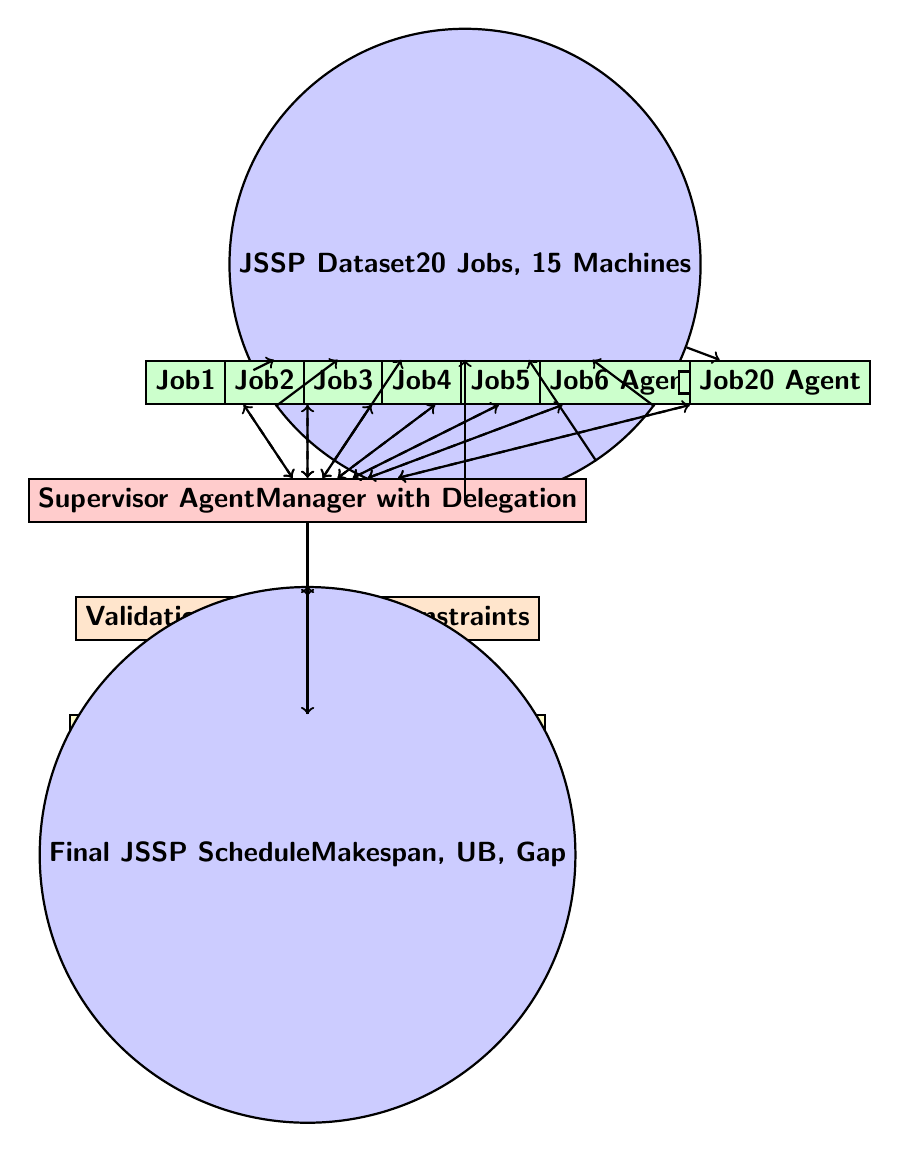
\begin{tikzpicture}[
    node distance=1.5cm,
    auto,
    thick,
    main node/.style={circle,fill=blue!20,draw,font=\sffamily\bfseries},
    agent node/.style={rectangle,fill=green!20,draw,font=\sffamily\bfseries},
    supervisor node/.style={rectangle,fill=red!20,draw,font=\sffamily\bfseries},
    validation node/.style={rectangle,fill=orange!20,draw,font=\sffamily\bfseries}
]

% Input
\node[main node] (input) {JSSP Dataset\\20 Jobs, 15 Machines};

% Job Agents (20 agents)
\node[agent node, below of=input, xshift=-3cm] (job1) {Job1 Agent};
\node[agent node, below of=input, xshift=-2cm] (job2) {Job2 Agent};
\node[agent node, below of=input, xshift=-1cm] (job3) {Job3 Agent};
\node[agent node, below of=input, xshift=0cm] (job4) {Job4 Agent};
\node[agent node, below of=input, xshift=1cm] (job5) {Job5 Agent};
\node[agent node, below of=input, xshift=2cm] (job6) {Job6 Agent};
\node[agent node, below of=input, xshift=3cm] (jobdots) {...};
\node[agent node, below of=input, xshift=4cm] (job20) {Job20 Agent};

% Supervisor Agent (Manager)
\node[supervisor node, below of=job1, xshift=1cm] (supervisor) {Supervisor Agent\\Manager with Delegation};

% Validation Agent
\node[validation node, below of=supervisor, xshift=0cm] (validation) {Validation Agent\\Check Constraints};

% Crew Process
\node[draw,rectangle,fill=yellow!20,below of=validation, xshift=0cm, minimum width=4cm] (crew) {CrewAI Process\\Sequential Delegation};

% Output
\node[main node, below of=crew] (output) {Final JSSP Schedule\\Makespan, UB, Gap};

% Arrows
\draw[->] (input) -- (job1);
\draw[->] (input) -- (job2);
\draw[->] (input) -- (job3);
\draw[->] (input) -- (job4);
\draw[->] (input) -- (job5);
\draw[->] (input) -- (job6);
\draw[->] (input) -- (job20);

\draw[->] (job1) -- (supervisor);
\draw[->] (job2) -- (supervisor);
\draw[->] (job3) -- (supervisor);
\draw[->] (job4) -- (supervisor);
\draw[->] (job5) -- (supervisor);
\draw[->] (job6) -- (supervisor);
\draw[->] (job20) -- (supervisor);

\draw[->] (supervisor) -- (validation);
\draw[->] (validation) -- (crew);
\draw[->] (crew) -- (output);

% Delegation arrows
\draw[<->,dashed] (supervisor) -- (job1);
\draw[<->,dashed] (supervisor) -- (job2);
\draw[<->,dashed] (supervisor) -- (job3);
\draw[<->,dashed] (supervisor) -- (job4);
\draw[<->,dashed] (supervisor) -- (job5);
\draw[<->,dashed] (supervisor) -- (job6);
\draw[<->,dashed] (supervisor) -- (job20);

\end{tikzpicture}
\caption{CrewAI Data Flow: Sequential Delegation with 22 Agents (20 Job + 1 Supervisor + 1 Validation)}
\label{fig:crewai_dataflow}
\end{figure}

% AutoGen Data Flow
\begin{figure}[h!]
\centering
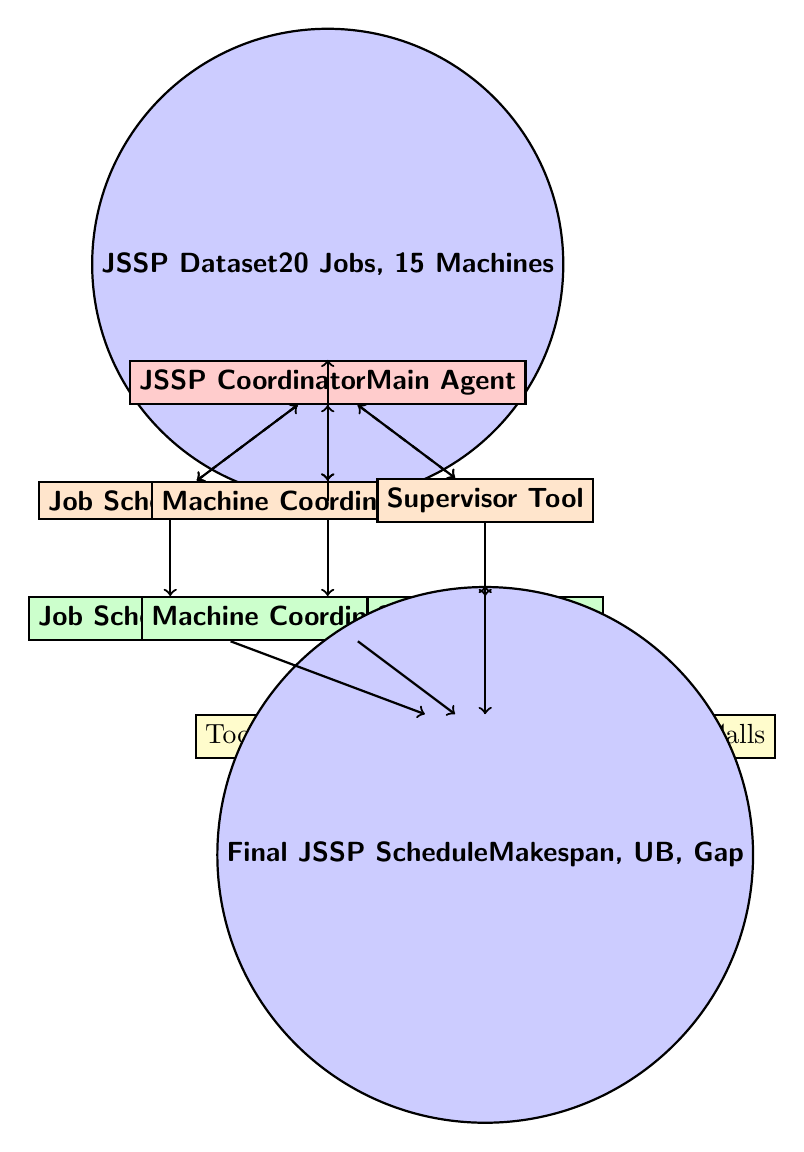
\begin{tikzpicture}[
    node distance=1.5cm,
    auto,
    thick,
    main node/.style={circle,fill=blue!20,draw,font=\sffamily\bfseries},
    agent node/.style={rectangle,fill=green!20,draw,font=\sffamily\bfseries},
    coordinator node/.style={rectangle,fill=red!20,draw,font=\sffamily\bfseries},
    tool node/.style={rectangle,fill=orange!20,draw,font=\sffamily\bfseries}
]

% Input
\node[main node] (input) {JSSP Dataset\\20 Jobs, 15 Machines};

% Coordinator
\node[coordinator node, below of=input] (coordinator) {JSSP Coordinator\\Main Agent};

% Tools
\node[tool node, below of=coordinator, xshift=-2cm] (job_tool) {Job Scheduler Tool};
\node[tool node, below of=coordinator, xshift=0cm] (machine_tool) {Machine Coordinator Tool};
\node[tool node, below of=coordinator, xshift=2cm] (supervisor_tool) {Supervisor Tool};

% Agents
\node[agent node, below of=job_tool] (job_agent) {Job Scheduler Agent};
\node[agent node, below of=machine_tool] (machine_agent) {Machine Coordinator Agent};
\node[agent node, below of=supervisor_tool] (supervisor_agent) {Supervisor Agent};

% Tool calls
\node[draw,rectangle,fill=yellow!20,below of=supervisor_agent, xshift=0cm, minimum width=4cm] (tool_calls) {Tool-Based Coordination\\Sequential Tool Calls};

% Output
\node[main node, below of=tool_calls] (output) {Final JSSP Schedule\\Makespan, UB, Gap};

% Arrows
\draw[->] (input) -- (coordinator);
\draw[->] (coordinator) -- (job_tool);
\draw[->] (coordinator) -- (machine_tool);
\draw[->] (coordinator) -- (supervisor_tool);

\draw[->] (job_tool) -- (job_agent);
\draw[->] (machine_tool) -- (machine_agent);
\draw[->] (supervisor_tool) -- (supervisor_agent);

\draw[->] (job_agent) -- (tool_calls);
\draw[->] (machine_agent) -- (tool_calls);
\draw[->] (supervisor_agent) -- (tool_calls);

\draw[->] (tool_calls) -- (output);

% Tool call arrows
\draw[<->,dashed] (coordinator) -- (job_tool);
\draw[<->,dashed] (coordinator) -- (machine_tool);
\draw[<->,dashed] (coordinator) -- (supervisor_tool);

\end{tikzpicture}
\caption{AutoGen Data Flow: Tool-Based Coordination with 3 Agents (Job Scheduler, Machine Coordinator, Supervisor)}
\label{fig:autogen_dataflow}
\end{figure}

% LangGraph Data Flow
\begin{figure}[h!]
\centering
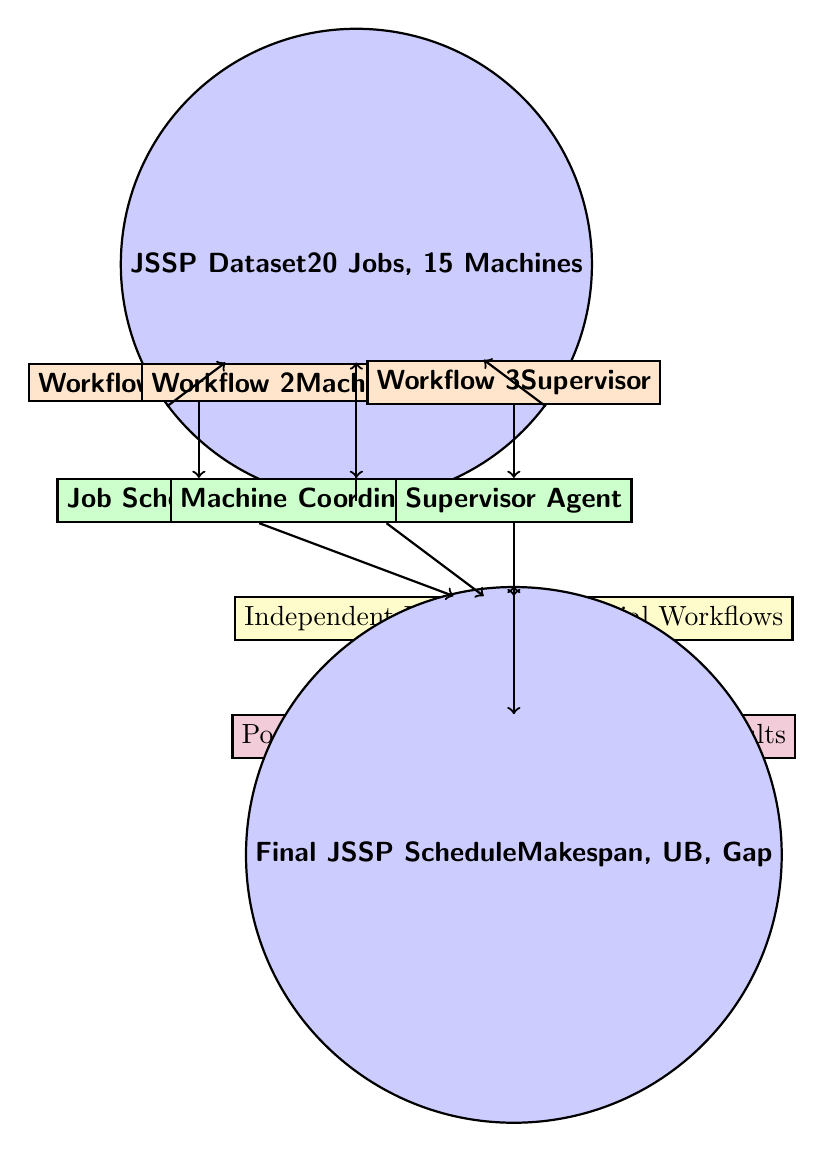
\begin{tikzpicture}[
    node distance=1.5cm,
    auto,
    thick,
    main node/.style={circle,fill=blue!20,draw,font=\sffamily\bfseries},
    agent node/.style={rectangle,fill=green!20,draw,font=\sffamily\bfseries},
    workflow node/.style={rectangle,fill=orange!20,draw,font=\sffamily\bfseries}
]

% Input
\node[main node] (input) {JSSP Dataset\\20 Jobs, 15 Machines};

% Independent Workflows
\node[workflow node, below of=input, xshift=-2cm] (workflow1) {Workflow 1\\Job Scheduler};
\node[workflow node, below of=input, xshift=0cm] (workflow2) {Workflow 2\\Machine Coordinator};
\node[workflow node, below of=input, xshift=2cm] (workflow3) {Workflow 3\\Supervisor};

% Agents
\node[agent node, below of=workflow1] (job_agent) {Job Scheduler Agent};
\node[agent node, below of=workflow2] (machine_agent) {Machine Coordinator Agent};
\node[agent node, below of=workflow3] (supervisor_agent) {Supervisor Agent};

% Independent execution
\node[draw,rectangle,fill=yellow!20,below of=supervisor_agent, xshift=0cm, minimum width=4cm] (independent) {Independent Execution\\Sequential Workflows};

% Aggregation
\node[draw,rectangle,fill=purple!20,below of=independent, xshift=0cm, minimum width=4cm] (aggregation) {Post-Execution Aggregation\\Combine Results};

% Output
\node[main node, below of=aggregation] (output) {Final JSSP Schedule\\Makespan, UB, Gap};

% Arrows
\draw[->] (input) -- (workflow1);
\draw[->] (input) -- (workflow2);
\draw[->] (input) -- (workflow3);

\draw[->] (workflow1) -- (job_agent);
\draw[->] (workflow2) -- (machine_agent);
\draw[->] (workflow3) -- (supervisor_agent);

\draw[->] (job_agent) -- (independent);
\draw[->] (machine_agent) -- (independent);
\draw[->] (supervisor_agent) -- (independent);

\draw[->] (independent) -- (aggregation);
\draw[->] (aggregation) -- (output);

\end{tikzpicture}
\caption{LangGraph Data Flow: Independent Workflows with 3 Agents (Job Scheduler, Machine Coordinator, Supervisor)}
\label{fig:langgraph_dataflow}
\end{figure}

% OpenAI Swarm Data Flow
\begin{figure}[h!]
\centering
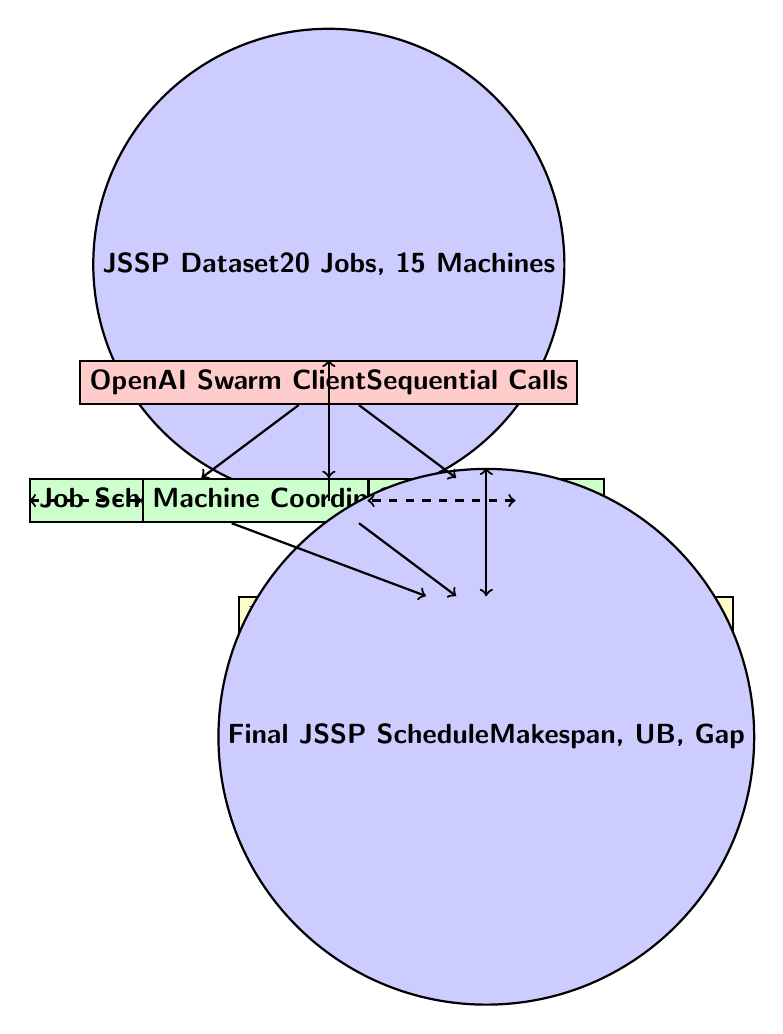
\begin{tikzpicture}[
    node distance=1.5cm,
    auto,
    thick,
    main node/.style={circle,fill=blue!20,draw,font=\sffamily\bfseries},
    agent node/.style={rectangle,fill=green!20,draw,font=\sffamily\bfseries},
    client node/.style={rectangle,fill=red!20,draw,font=\sffamily\bfseries}
]

% Input
\node[main node] (input) {JSSP Dataset\\20 Jobs, 15 Machines};

% Client
\node[client node, below of=input] (client) {OpenAI Swarm Client\\Sequential Calls};

% Agents
\node[agent node, below of=client, xshift=-2cm] (job_agent) {Job Scheduler Agent};
\node[agent node, below of=client, xshift=0cm] (machine_agent) {Machine Coordinator Agent};
\node[agent node, below of=client, xshift=2cm] (supervisor_agent) {Supervisor Agent};

% Message passing
\node[draw,rectangle,fill=yellow!20,below of=supervisor_agent, xshift=0cm, minimum width=4cm] (messages) {Message Passing\\Sequential Client Calls};

% Output
\node[main node, below of=messages] (output) {Final JSSP Schedule\\Makespan, UB, Gap};

% Arrows
\draw[->] (input) -- (client);
\draw[->] (client) -- (job_agent);
\draw[->] (client) -- (machine_agent);
\draw[->] (client) -- (supervisor_agent);

\draw[->] (job_agent) -- (messages);
\draw[->] (machine_agent) -- (messages);
\draw[->] (supervisor_agent) -- (messages);

\draw[->] (messages) -- (output);

% Message passing arrows
\draw[<->,dashed] (job_agent) -- (machine_agent);
\draw[<->,dashed] (machine_agent) -- (supervisor_agent);

\end{tikzpicture}
\caption{OpenAI Swarm Data Flow: Sequential Client Calls with 3 Agents (Job Scheduler, Machine Coordinator, Supervisor)}
\label{fig:swarm_dataflow}
\end{figure}

% Summary Table
\begin{table}[h!]
\centering
\caption{Multi-Agent Framework Comparison}
\label{tab:framework_comparison}
\begin{tabular}{|l|c|c|c|c|}
\hline
\textbf{Framework} & \textbf{Agent Count} & \textbf{Architecture} & \textbf{Data Flow} & \textbf{Coordination} \\
\hline
MAPLE & 22 (20 Job + 1 Supervisor + 1 Validation) & 3-layer with dependency management & Context sharing + sequential execution & Dependency-based with validation \\
\hline
CrewAI & 22 (20 Job + 1 Supervisor + 1 Validation) & Sequential delegation & Internal delegation & Supervisor manages other agents \\
\hline
AutoGen & 3 (Job Scheduler, Machine Coordinator, Supervisor) & Tool-based coordination & Tool calls with result aggregation & Main coordinator uses agents as tools \\
\hline
LangGraph & 3 (Job Scheduler, Machine Coordinator, Supervisor) & Independent workflows & Independent execution + post-aggregation & Post-execution aggregation \\
\hline
OpenAI Swarm & 3 (Job Scheduler, Machine Coordinator, Supervisor) & Sequential client calls & Message passing between agents & Direct message passing \\
\hline
\end{tabular}
\end{table}

\end{document}
